
\documentclass[10pt,letterpaper]{article}

\usepackage{cogsci}

\cogscifinalcopy % Uncomment this line for the final submission 

\usepackage[
    backend=biber,
    style=apa,
    natbib=true,
    doi=false,
    isbn=false,
    url=false,
]{biblatex}
\addbibresource{refs.bib}
\setlength{\bibhang}{.125in}

\usepackage{dblfloatfix}    % To enable figures at the bottom of page
\usepackage{graphicx}
\usepackage{pslatex}
\usepackage{float} 

%\usepackage[none]{hyphenat} % Sometimes it can be useful to turn off
%hyphenation for purposes such as spell checking of the resulting
%PDF.  Uncomment this block to turn off hyphenation.


\usepackage{mathtools}
% \usepackage{subcaption}
\usepackage{amsmath}
\usepackage{amssymb}
\usepackage{bm}% http://ctan.org/pkg/bm % for italic bold math

\usepackage{hyperref}
\PassOptionsToPackage{dvipsnames,table}{xcolor}
\usepackage{xspace}
\xspaceaddexceptions{]\}}

\DeclareMathOperator*{\argmax}{arg\,max}

\DeclareMathOperator{\E}{\operatorname {E}}
\let\P\relax
\DeclareMathOperator{\P}{\operatorname {P}}

\DeclareMathOperator{\Corr}{Corr}
\DeclareMathOperator{\Cov}{Cov}

\DeclareMathOperator{\Like}{\mathcal{L}}
\DeclareMathOperator{\Lagr}{\ell}

% \renewcommand{\vec}[1]{\underline{#1}}

\newcommand{\emol}[1]{\emph{\MakeUppercase #1}}
\newcommand{\feature}[1]{\texttt{#1}}

\newcommand{\C}{\texttt{C}\xspace}
\newcommand{\D}{\texttt{D}\xspace}
\newcommand{\CC}{\texttt{CC}\xspace}
\newcommand{\CD}{\texttt{CD}\xspace}
\newcommand{\DC}{\texttt{DC}\xspace}
\newcommand{\DD}{\texttt{DD}\xspace}

\usepackage[dvipsnames]{xcolor}

%\setlength\titlebox{4.5cm}
% You can expand the titlebox if you need extra space
% to show all the authors. Please do not make the titlebox
% smaller than 4.5cm (the original size).
%%If you do, we reserve the right to require you to change it back in
%%the camera-ready version, which could interfere with the timely
%%appearance of your paper in the Proceedings.


\title{Reasoning about the antecedents of emotions:\\Bayesian causal inference over an intuitive theory of mind}
 
\author{{\large {\bf Sean Dae Houlihan}{\normalfont\textsuperscript{1} (daeda@mit.edu)}}, {\large {\bf Desmond Ong}{\normalfont\textsuperscript{2} (dco@comp.nus.edu.sg)}},\\{\large {\bf Maddie Cusimano}{\normalfont\textsuperscript{1} (mcusi@mit.edu)}}, {\large {\bf Rebecca Saxe}{\normalfont\textsuperscript{1} (saxe@mit.edu)}} \\
{\normalfont\textsuperscript{1}}Brain and Cognitive Sciences, Massachusetts Institute of Technology\\
{\normalfont\textsuperscript{2}}Department of Information Systems and Analytics, National University of Singapore
%{\normalfont\textsuperscript{3}}Institute of High Performance Computing, A*STAR Singapore
}

\begin{document}

\maketitle

\begin{abstract}

It is commonly believed that expressions visually signal rich diagnostic information to human observers. We studied how observers interpret the dynamic expressions that people spontaneously produced during a real-life high-stakes televised game. We find that human observers are remarkably poor at recovering what events elicited others' facial and bodily expressions. Beyond simple inaccuracy, people's causal reasoning exhibits systematic model-based patterns of errors. We show that latent emotion representations can explain people's reasoning about the unseen causes of expressions. A hierarchical Bayesian model simulates which events people infer to be the cause of others' expressions by comparing the emotions inferred from the expressions against the emotions people were predicted to experience in various situations. This causal model provides a close, parameter-free fit to human causal judgments, suggesting that humans interpret expressions in the context of emotion predictions generated by a causally-structured mental model of other minds.


\textbf{Keywords:} 
emotion understanding; intuitive theory; affective cognition; causal reasoning; emotion recognition
\end{abstract}


\section{Introduction}

A common assumption in psychology and machine learning research is that human observers and emotion recognition algorithms can decode emotions from people's facial and bodily expressions \citep[for review, see][]{barrett2019reconsidered}. Here we use evidence from an experiment in human observers, and a close quantitative fit using a Bayesian belief updating model, to argue instead that human observers understand others' emotions by reasoning over a causally structured intuitive theory of mind. 

The problem of understanding someone's emotional experience can be framed as perceptual pattern matching.
On this view, expressions can signal someone's current emotional state, intentions, and assessments of the eliciting situation \citep{keltner2019betadvances, shariff2011cdps}. 
Thus, with perceptual access to the relevant expression cues, observers should be able to reliably identify others' emotions \citep{cowen2020face28}. This ``{\em emotion recognition}'' view aligns with people's lay intuitions. For example, observers expect that intensely positive and intensely negative experiences should lead to highly distinctive facial expressions \citep{aviezer2012science}.

In the view of {\em emotion recognition}, people can decode causal antecedents from patterns of expressive behavior. For example, it is argued that observers can reliably map between expressions, emotions, and situations. Observers may be given a photo and asked to identify what events evoked the expression \citep{haidt1999ce}, or label the expression with an emotion word \citep{tracy2004ps}. Similarly, observers may be given a description of events and asked to select which expression matches that situation \citep{cordaro2020facebody}. 
This view assumes that emotion knowledge reflects a common network of associations, which allows observers to relate expressions, emotions, and events. 

However, a growing body of evidence shows that isolated expressions are surprisingly ambiguous. Human observers are unable to distinguish genuine facial expressions spontaneously produced during highly desirable experiences (e.g. the surprise homecoming of a deployed family member) from expressions produced during highly aversive experiences (e.g. being a bystander to a terrorist attack) \citep{wenzler2016pleasurepain, israelashvili2019dynamicambig}.
This unintuitive result is highly replicable \citep{camerer2018manylabsnatsci} and suggests that expressions alone are insufficient to explain how humans infer others' emotions in naturalistic settings. 

In light of evidence that the perceptual information conveyed by expressions is not sufficient to account for human emotion understanding, several groups have proposed that, instead of ``recognizing'' emotions in expressions, observers ``reason'' about others' emotions using a mental model of other minds. 
In this ``{\em emotion reasoning}'' view, human observers interpret expressions by reasoning about what causal explanation jointly maximizes the probability of events, emotions, and the expressions.
Multiple sources of emotion-relevant information can be integrated in an inference over an intuitive theory of mind \citep{saxe2017cop, ong2015cueint, ong2019topics, hoegen2019emoreg, wu2018childinvplan, freemanambady2011dynamicinteractive}. 
Indeed, there is strong evidence that observers incorporate contextual information about events when interpreting expressions \citep{aviezer2012science, kayyal2015context, anzellotti2021emotion}. 

In the view of {\em emotion reasoning}, 
cues about the situation might lead to emotion predictions that conflict with the emotions someone appears to express. For example, cues about the event context can generate confident emotion predictions that shape the inference of emotions from expressions \citep{anzellotti2021emotion, ong2015cueint}. Similarly, observers integrate someone's expression with her actions to infer her intentions, appraisals, and future behavior \citep{demelo2014readingmindsexpressions}.
This view suggests that emotion understanding involves integrating multiple sources of, often conflicting, perceptual and conceptual information to infer unknown causes from observed reactions. Building on the theoretical foundations laid by this prior work, we present a model of how people reason about which events are a likely causal explanation for another's expressions. To our knowledge, this is the first formal model of abductive inference over emotions.

The two frameworks, {\em emotion recognition} and {\em emotion reasoning}, make distinct predictions regarding the patterns of errors human observers will tend to make.
If emotion understanding is best thought of as perceptual pattern matching, 
judgments may be noisy, especially when the perceptual signal is degraded because an expression is partially occluded, low resolution, or changes rapidly.
By contrast, if emotion understanding is better thought of as model-based causal reasoning, 
judgments are likely to exhibit peaked failure modes rather than non-specific noise \citep{kruger1999naivecynicism, gopnik1993selfknowledge, saxe2005argumentfromerror}.
Inaccuracies in the intuitive theory are likely to generate model-based errors---systematic interactions between observations and an intuitive theory that poorly reflects the properties of the world \citep{gopnik1994theorytheory}. 


There are several requirements of a paradigm that aims to compare the predictions of {\em emotion recognition} 
against the predictions of {\em emotion reasoning}. 
The expression stimuli should provide perceptually rich veridical information (as opposed to isolated static faces of posed expressions or computer-generated avatars). The design should afford an objective measure of ground truth accuracy (so that `errors' are well defined). And the task should allow noisy judgments arising from perceptually ambiguous stimuli to be differentiated from systematically incorrect judgments. In the following sections we describe a novel experimental paradigm designed to meet these criteria.


First, we show that human observers are remarkably poor at recognizing the content of others' actual experiences from their expressions, even when the perceptual information is dynamic, includes faces and bodies, and is spontaneously produced during real high-stakes situations. 
Moreover, we find that these errors are systematic.
Next, we show that a parameter-free Bayesian model can capture which events observers inferred to be the cause of these expressions. The {\em emotion reasoning} model combines predictions of the emotions others are likely to experience in various situations, with the emotions they are inferred to experience from their expressions.
Finally, we compare the causal inferences simulated under the assumptions of {\em emotion reasoning}, with the causal inferences simulated under the assumptions of {\em emotion recognition}. The model of {\em emotion reasoning} predicts the pattern of human causal judgments substantially better than the model of {\em emotion recognition}.




%%%%%%%%%%%%%%%%%%%

\subsection{Stimulus generation: spontaneous expressions in a real-life high-stakes social dilemma}

We artificially separated the perceptual information from context information in recordings of a televised British gameshow called {\em GoldenBalls}.
Every episode of GoldenBalls culminates with two contestants playing a dramatic one-shot instantiation of the Prisoner's Dilemma. Each player is given a choice to ``Split'' or ``Steal'' a jackpot (in standard Prisoner's Dilemma notation, to ``\C{}ooperate'' or ``\D{}efect'', respectively). If both decide to ``\C{}ooperate'', they each receive half of the jackpot. 
If one player instead chooses ``\D{}efect'', that player wins the entire jackpot and the other player who chose ``\C{}ooperate'' leaves with nothing. If both players choose ``\D{}efect'', both get nothing\footnote{\citet{rapoport1988weakpd} defines this payoff structure as a Weak Prisoner's Dilemma because the \CD payoff confers the same monetary reward (\$0) to player 1 as the \DD payoff. Thus, with respect to a player's first-person financial payout, defecting is never harmful, but is only conditionally beneficial.}. 
Players negotiate with each other in front of a live audience in an attempt to convince the other to make a choice that is financially disadvantageous (to cooperate). Each player makes a decision in private, then they simultaneously reveal their choices, all while being filmed.

The game is emotionally evocative by design. When the choices are revealed, players discover whether they have won or lost real and often substantial sums of money; and whether they have successfully cooperated, successfully duped, been duped by, or failed to dupe the other player. The TV cameras capture their spontaneous unscripted dynamic expressions, including changes of posture and expression of players' faces, shoulders, upper bodies, and hands.

We extracted 88 unique 5-second videos, each depicting a single player's expressions, by splicing together footage from the moments surrounding the climactic reveal)\footnote{Demos are available on the project's \texttt{github} repository.}.
%\footnote{Demos available at \href{https://github.com/daeh/emo-reasoning-cogsci22}{github.com/daeh/emo-reasoning-cogsci22}.}.
The four outcomes were represented equally in the stimuli (N=22 for each outcome), reflecting the true distribution of play---across all 287 broadcast episodes, players were 53\% likely to cooperate \citep{vandenAssem2012goldenballs}, and the decisions of a player dyad (the two opposing players in the game) were statistically independent of each other \citep{burtonchellew2012goldenballs}.
Each video silently showed a single person anticipating and reacting to a game outcome, but overt cues as to the players' decisions and the outcome of the game were masked.
The average size of the jackpot was \$25,582.58% USD.


\section{Systematic errors in human causal reasoning about the antecedents of emotional expressions}

Every dataset used in this paper was collected on Amazon mTurk. We restricted workers by geolocation to the United States using mTurk credentials and asked workers to only begin the experiment if they were fluent in English. Workers who reported any familiarity with the GoldenBalls gameshow were excluded from analysis.


\subsection{Experiment~1: Outcome judgments}

Observers first watched an introductory video explaining the rules of the game. Then, over 88 trials, they were shown each 5-second expression video along with the corresponding pot size, and asked to guess which decision each player had made. Players either chose to \C{}ooperate or to \D{}efect, leading to four possible outcomes ($a$) for the dyad, denoted \CC, \CD, \DC, \DD. For instance, \CD indicates that the focal player \C{}ooperated, while the opposing player \D{}efected. The actual decisions associated with each video provide a ground-truth measure of accuracy. 


\vspace{1 mm}
\noindent\textbf{Results}
A group of N=93% adults (46% female) classified the 88 videos into four outcome categories (chance=25\%) and indicated their confidence about each player's choice on a 3-point scale. Each observer responded to every video.
On average, observers performed above chance but made many errors, inferring the correct outcome for an average of
36.6\% [35.0, 38.1]% of the videos (95\% bootstrap CI estimated by resampling observers). This corresponds to a
median F-score (macroaveraged across the four outcome-categories) of 0.350 [0.335, 0.361]%, which is low but significantly greater than chance (two-sided Wilcoxon signed-ranks test, $z = 7.945$, $p < 0.001$%). 
The null distribution was estimated by shuffling outcome judgments within observers.

Observers' classification performance was highly heterogeneous across outcome-categories (Figure~\ref{fig:fscore}). When the two players had, in reality, chosen to Split the pot (\CC), observers accurately classified 54.1\% [50.7, 57.4]% of videos on average (median F-score and Wilcoxon test: 0.517 [0.491, 0.540]%, $z = 8.224$, $p < 0.001$%).
 By contrast, when both players had, in reality, tried to Steal the pot (\DD), observers accurately classified only 
 15.9\% [13.2, 18.9]% of videos on average, substantially \emph{below} chance (F-score~=~0.146 [0.121, 0.182]%, $z = -4.041$, $p < 0.001$%). 
Relative to their other judgments, when observers were maximally confident about both players' actions\footnote{
Observers reported maximum confidence for 30.9\%% of their outcome judgments.
}, they showed better classification performance for \CC and \CD videos (within observer, two-sided Wilcoxon test; \CC: $z = 7.127$, $p < 0.001$%; \CD: $z = 6.302$, $p < 0.001$%). Confidence was not related to performance for \DC videos ($z = -1.700$, $p = 0.089$%). For \DD videos, confidence was \textit{inversely} related to performance ($z = -4.515$, $p < 0.001$%).


%%%%%%%%%%%%%%
\begin{figure}[tb]
    \centering
    {%
      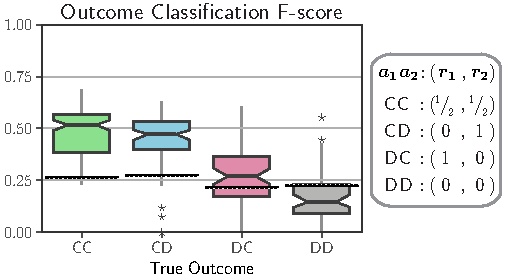
\includegraphics[width=1.0\columnwidth]{fig/f1comp-cogsci2022.pdf}%
    }
    \caption{
    \textbf{Outcome judgments from expressions.}
    Observers viewed player~1's reaction to learning the outcome of the game and inferred which choice (\C or \D) both players in the dyad had made.
    The F-scores of observers' classification judgments are shown grouped by the true outcome of the games. 
    Notches indicate 95\% bootstrap CI. Dashed lines indicate the median level of chance performance, given the observer-level response biases.
    % The actions chosen by the two players in a dyad determine the players' financial rewards.
    The legend gives the four possible outcomes (an outcome $a$ comprises $a_1$ and $a_2$, which indicate the action chosen by player~1 and player~2) and the associated monetary rewards ($r_1$ and $r_2$ indicate the proportion of the jackpot paid to player~1 and player~2).
    }
    \label{fig:fscore}
\end{figure}


\vspace{1 mm}
\noindent\textbf{Summary}
Observers performed poorly when asked to recover the true event antecedents, despite viewing stimuli that, according to the {\em emotion recognition} account, should be most informative: spontaneous dynamic facial and bodily expressions recorded in real high-stakes situations. 
Accuracy is straightforward to measure in this task and does not depend on the experimenter's normative assumptions: it is simply the proportion of videos for which observers correctly inferred the game outcome. 
No observer correctly classified more than 53\% of the videos. 
Observers reliably, confidently, and incorrectly inferred that the expressions of players in \DD games were reactions to other outcomes. 





\section{Emotion judgments}

We propose that observers infer which events evoked observed expressions by reasoning over a causally-structured intuitive theory of other minds. 
In Experiment~1, observers performed the naturalistic task of guessing what unobserved event elicited someone's spontaneous expression. 
We hypothesize that observers infer events from expressions via latent representations of emotion.
In order to test if we could explain the outcome judgments in Experiment~1 as causal reasoning over emotion latents, we next collected emotion judgments from independent groups of observers: Datasets~2 and 3 will be used to explain outcome judgments in this experiment (Dataset~1), but are not analyzed independently.

\subsection{Dataset~2: Emotion predictions}

We directly measured what emotions observers expected players to experience across a range of specific event contexts. After watching the introductory video that explained the rules of the game, observers predicted the emotions experienced by players on the gameshow. In each trial, observers were shown the size of the jackpot, the choice made by the focal player, the choice made by the opposing player, how much money each player won, and a still photo of the focal player taken before the players' choices were revealed (observers did not see the players' reactions to the outcome of the game).
All of the information given on a trial 
reflected what actually happened on the gameshow. 

An independent group of N~=~164% English-speaking adults (74% female) was shown descriptions of 12 out of 88 games, then asked to predict emotions that the focal player experienced.
Observers predicted the focal player's emotional experience, using continuous scales to report the intensity of 20 different emotions. 
We estimated inter-rater reliability by comparing the emotion predictions of one observer with the mean emotions that other observers predicted for the same players. 
Across emotions and players, the median Pearson correlation and 95\% bootstrap confidence interval (CI) was $r=$~0.66 [0.62, 0.70]%, indicating that independent observers made similar predictions of players' emotion experiences.



\subsection{Dataset~3: Emotion attributions}


We directly measured observers' attributions of emotions to the expressions of players in the GoldenBalls videos. 
An independent group of English-speaking adults (N=135%, 58% female) judged the players' emotions from the 5-second video stimuli. Observers began the experiment by watching the introductory video, then judged the emotions of 12 players. Each trial provided the pot size but not the players' actions. Observers judged how much the focal player was experiencing the twenty different emotions. 
As in Dataset~2, emotion judgments were reliable across emotions and videos, with a median correlation of $r=$ 0.66 [0.64, 0.69]% between one observer and the mean of other observers' attributions to the same players.



\begin{figure*}[tb]
    \centering
    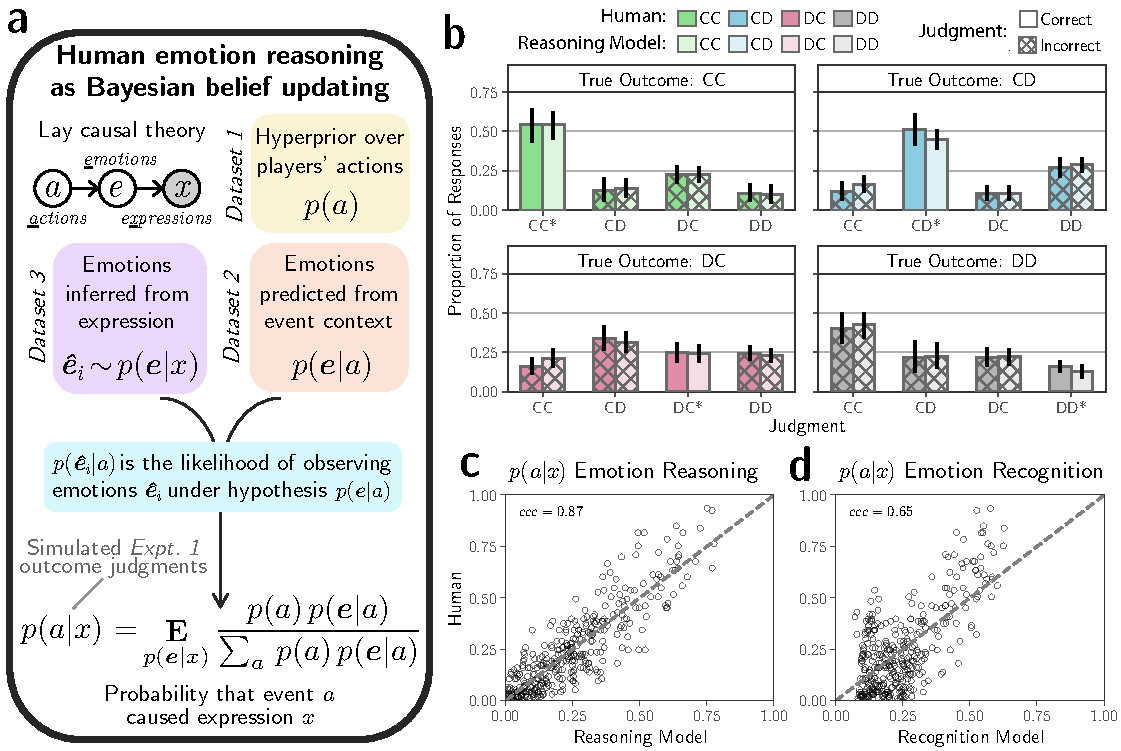
\includegraphics[width=\textwidth]{fig/bor-cogsci2022.pdf}
    \caption{
    \textbf{Bayesian model of human emotion reasoning}. \textbf{(a)} Schematic depiction of the model. Observers infer which events elicited the observed expressions by reasoning over latent representations of emotion.
    \textbf{(b)} Outcome judgments of human observers and the {\em emotion reasoning} model, grouped by ground-truth. Correct judgments are indicated by asterisks and solid bars.
    E.g. Observers incorrectly guessed that the expressions of players from \DD games (bottom right cell) were from \CC games more than the correct outcome. Error bars give 95\% bootstrap CI.
    \textbf{(c)} Outcome judgments simulated under {\em emotion reasoning} assumptions, where the $p(\bm{e}|x)$ and $p(\bm{e}|a)$ distributions reflect separate information. 
    \textbf{(d)} Outcome judgments simulated under {\em emotion recognition} assumptions, where $p(\bm{e}|x)$ and $p(\bm{e}|a)$ reflect common information.
    }
    \label{fig:bor_composit}
\end{figure*}

\section{Causal reasoning over latent emotion representations in a hierarchical Bayesian belief-updating model} 

We propose that the observers in Experiment~1 inferred outcomes by reasoning about what hypothetical event was the best causal explanation for the observed expressions. This inference reflects the intuitive theory that emotions are reactions to antecedent events, and that expressions are caused by emotions (~$a \rightarrow e \rightarrow x$~; Figure~\ref{fig:bor_composit}). 


We simulated observers' outcome predictions as inference in an intuitive theory of mind, where observers use the emotions they infer from players' dynamic expressions \( p(\bm{e}|x) \), and the emotions they expect players to experience in the possible outcomes \( p( \bm{e}|a ) \) (where \( a \in \big\{ \CC, \CD, \DC, \DD \big\} \)), to infer which outcome was most likely to have generated the observed expressions (Figure~\ref{fig:bor_composit}a). This corresponds to inferring the posterior distribution $p(a|x)$, which can be computed by marginalizing out emotion from the joint distribution $p(a,\bm{e}|x) = p(a|\bm{e})p(\bm{e}|x)$, noting that actions and expressions are conditionally independent given emotions.  
\begin{equation}\label{eq:boring-expectation}
    \begin{split}
        p(a|x) \ =\  \int_{\bm{e}} &p(\, a\, |\, \bm{e}\, ) \, p(\, \bm{e}\, |\, x\, )\, \mathrm{d}\bm{e} \ \: =\ \mathop{\E}_{p(\, \bm{e}\, |\, x\, )} p(\, a\,  |\,  \bm{e} \, )\\ 
        &\text{where }\,\, p(\, a\, |\, \bm{e}\, ) \propto p(a) \, p(\, \bm{e}\, |\, a\, )
    \end{split}
\end{equation}


We model observers' mental distribution of emotions given expressions, $p(\bm{e}|x)$, as the empirical distribution of emotion judgments $\hat{\bm{e}}_i$. To approximate the expectation in Equation~\ref{eq:boring-expectation}, we sum over the responses from the $N_x$ observers (indexed by $i$) who attributed emotions to expression $x$ in Dataset~3. 
\begin{equation}
    \begin{split}
        p(a|x) = \frac{1}{N_x} &\sum_{i}^{N_x}{ \: p(\,a \, | \, \hat{\bm{e}}_i \, ) } \\
        \text{where }\,\,
        p(a \, | \, \hat{\bm{e}}_i) &= \frac{p(a) \: p(\, \hat{\bm{e}}_i\, |\, a \,)}{\sum_{a} \: {p(a) \: p(\, \hat{\bm{e}}_i \, | \, a \,)}}
    \end{split}
\end{equation}



We model observers' mental distribution of emotions elicited by players' actions, $p(\bm{e}|a)$, based on the emotion predictions $\hat{\bm{e}}_j$ from game descriptions (comprising an outcome, pot size, and player photo). We use the responses from the $N_a$ observers (indexed by $j$) who were shown game descriptions $c$ with outcome $a$ in Dataset~2, to construct a weighted Kernel Density Estimate (KDE) of the emotions observers expect.
We weight each response by $w_j = (V_{a}N_{c_j})^{-1}$ to account for the number of observers who saw each description ($N_{c_j}$), and the number of videos $V_a$ with outcome $a$.
%
\begin{align} \label{eq:borkernel}
    p(\bm{e}|a) &= \sum^{N_a}_{j} w_j \mathcal{N}(\bm{e} ; \  \mu=\hat{\bm{e}}_j, \bf{\sigma}\mathit{I})
\end{align}

The KDE estimates the population's marginal distribution \( p(\bm{e}|a) \) (the emotions players were predicted to experience) as a weighted mixture of Gaussian kernels, where the vector \( \bf{\sigma} \) is the kernel bandwidths corresponding to the 20 emotions and \( \mathit{I} \) is the 20-dimensional identity matrix.
The kernel bandwidth was calculated for each emotion based on the sample standard deviation using Scott's Rule \citep{scott1992}.


The hyperprior over the actions chosen by a player dyad, $p(a)$, was estimated from observers' meta-knowledge about other observers\footnote{
Observers in Experiment~1 were asked to estimate how other observers would judge the expressions (e.g. ``what percentage of people would guess that this player cooperated?''). 
We used observers' guesses of the population's judgments to estimate the population's joint action hyperprior $p(a)$.
} (not from the outcome judgments to be explained).
Finally, the resulting posterior $p(a|x)$ gives the distribution of responses over outcome-categories, i.e.
the simulated probability of observers inferring that expression $x$ was elicited by outcome $a$.



\vspace{1 mm}
\noindent\textbf{Results}
The {\em emotion reasoning} (Figure~\ref{fig:bor_composit}a) model predicted observers' overall accuracy with respect to ground truth: accuracy and 95\% bootstrap CI, human~=~36.6\% [32.8, 40.3]%, model~=~33.9\% [31.0, 36.9]%.
Comparing the human and {\em emotion reasoning} model judgments for the predicted and ground-truth outcomes reveals a close match across all categories (Figure~\ref{fig:bor_composit}b). 
Observers tended to infer the correct outcome from players' expressions in \CC games. 
When \CC videos were misclassified, observers tended to choose the other outcome that would confer a financial reward (\DC), more often than the outcomes in which the player would receive nothing (\CD or \DD). Observers also tended to classify \CD videos correctly. The most common error was to misclassify \CD video as the financially similar \DD outcome (both confer the minimum payoff to the focal player).
In contrast with videos from \CC and \CD games, people did not tend to correctly classify \DC videos. Observers inferred that \DC videos showed players in \CD games more often than the true outcome. 

Observers overwhelmingly inferred that the expressions made by players in \DD games (where both players defect and leave with nothing) were produced by players experiencing \CC outcomes (where both players cooperate and share the jackpot). 
Interestingly, for \DD videos, the correct outcome was the least popular judgment. It may seem surprising that observers systematically misclassify \DD videos as \CC, but this is precisely the pattern predicted by the model.


Figure~\ref{fig:bor_composit}c details the stimulus-level data depicted in Figure~\ref{fig:bor_composit}b. Each point corresponds to a video-outcome, e.g. the proportion of \DD judgments that the model expects versus the proportion of \DD judgments by people, for a given video (regardless of ground truth). The model accurately captured the empirical data (concordance correlation coefficient $ccc$~=~0.869 [0.841, 0.904]%; Pearson $r$~=~0.877 [0.849, 0.910]%, 95\% bootstrap CI were estimated by resampling stimuli with replacement across outcomes). 
Lin's Concordance Correlation Coefficient penalizes deviations from the identity line (perfect prediction), making it a more stringent metric of explanatory power than Pearson's correlation \citep{lin1989concordance}.


\subsubsection{\large Simulation under {\em ``recognition''} assumptions}

The {\em recognition} model reflects the belief that rich perceptual expression signals are the primary source of reliable emotion information. 
In {\em emotion recognition}, emotion knowledge reflects a common network of statistical associations. Rich perceptual access to expressions should allow observers to make accurate inferences of emotions, intentions, and the eliciting situations. 
%To simulate outcome judgments under ``recognition'' assumptions, we treat the interpretation of expressions (Dataset~3) as observers' noisy accurate emotion knowledge. 
This implies that observers make accurate inferences of emotions from expressions, and have an accurate understanding of what emotions players will appear to express in reaction to the game's outcomes.


Recall that in the {\em reasoning} model, emotions predicted given event descriptions \( p(\bm{e}|a) \) can reflect different information than emotions attributed given the expressions of players experiencing those events \( p(\bm{e}|x) \).
In the {\em recognition} model, we instantiate the assumption that observers have a noisy but accurate understanding of what emotions players who experience outcome $a$ will appear to express. 
This is accomplished by
replacing the emotions predicted for an outcome, \( p(\bm{e}|a) \), with a KDE formed from the emotions attributed to the expressions of players reacting to that outcome.
Thus, whereas in the {\em reasoning} model, observers' emotion knowledge about outcome $a$ is estimated from descriptions of the $a$ games (Dataset~2),
in the {\em recognition} model, observers' emotion knowledge about outcome $a$ is estimated from expressions of players who actually experienced $a$ games (Dataset~3). 
The {\em recognition} model therefore does not use Dataset~2. 
Rather, Dataset~3 is used to estimate both latent emotion distributions.


\vspace{1 mm}
\noindent\textbf{Results}
Outcome judgments simulated under the assumptions of {\em emotion recognition}
captured the empirical data less effectively\footnote{
Whereas the {\em reasoning} model is parameter-free, for the {\em recognition} model, the kernel bandwidth was fit in order to estimate the upper extent of how well the model can capture human judgments.
}
(Figure~\ref{fig:bor_composit}d; concordance correlation coefficient $ccc$~=~0.655 [0.610, 0.707]%; Pearson $r$~=~0.713 [0.661, 0.774]%). 

\vspace{1 mm}
\noindent\textbf{Model comparison}
The {\em reasoning} model assumes that observers adjudicate between alternative causal hypotheses by comparing the emotions a player appeared to express against emotions an outcome was predicted to evoke. The {\em recognition} model assumes that observers have an accurate understanding of what emotions players will appear to express in each outcome, and perceptually match a player's emotional expression to the pattern associated with the eliciting outcome.
The Bayes Factor indicates that observers' outcome judgments are %$10^{386}$% 
$>10^{10}$ times more likely under the {\em reasoning} model than under the {\em recognition} model.

%Observers might report that winning an Olympic gold medal is likely to make someone joyful and proud. But when observers see the athlete crying, the nuances of her expressions will convey that she is experiencing a desirable positive situation, leading observers to accurately conclude that she won. 


\section{Discussion}

Behavioral results and a quantitative model provide strong support for {\em emotion reasoning}: observers make errors because they systematically misinterpret the meaning of expressions, and thus independent observers reliably and confidently endorse the same incorrect outcome judgments.
The agreement between the predictions of the {\em emotion reasoning} model and the classification pattern generated by human observers supports our proposal that people use a sophisticated intuitive theory of mind to reason about others' emotions. 

The causally-structured intuitive theory incorporates emotion concepts and expression cues. The emotions that players were expected to experience, and the emotions they appeared to express, were sufficient to capture key patterns of how human observers causally reasoned about unseen events. Importantly, no reference to emotion was made in Experiment~1; %(the empirical judgments to be matched); 
observers were not cued to think about emotions when they guessed what outcomes players experienced. Yet, the {\em reasoning} model successfully predicted what outcome judgments observers made by reasoning over latent representations of emotions, which were supplied by independent observers. % (Datasets~2 and 3).
Thus, the %20-dimensional 
emotion judgments we collected contain richly structured social information sufficient to capture observers' reasoning about the causal connection between unobserved events and others' emotional expressions. By contrast, the {\em recognition} model, which simulates observers' emotion understanding as perceptual pattern matching over a common network of statistical associations, failed to closely capture the empirical pattern of outcome judgments.

%%%%%%%%%%%%

These results are consistent with prior work measuring how observers infer event antecedents from genuine spontaneous expressions. \citet{albanie2016dealnodeal} showed human observers dynamic facial expressions spontaneously produced during a high-reward televised gameshow; the observers were asked to judge whether the event immediately preceding the expression had been financially good or bad for the players. 
In the binary forced-choice, observers achieved 62\% classification accuracy on average, corresponding to an average ROC-AUC of 0.71 [0.66, 0.76], above chance but with many errors. Despite using perceptually richer expressions, observers in the present study were not more successful at inferring event antecedents\footnote{Binary ROC-AUC~=~0.58 [0.57, 0.59]%.}: observers were unable to reliably differentiate the expressions of players who won money (\CC and \DC) from the expressions of players who did not (\CD and \DD).
Thus even rich perceptual access to dynamic videos of genuine expressions in real high stakes situations does not allow observers to reliably recognize the true events that elicited them.

A key characteristic of the current experimental paradigm is that it affords analysis of a complex pattern of causal inferences (a $4 \times 4$ matrix of {\em inferred}~$\times$~{\em veridical} outcomes) where errors are objectively defined. The event categories are distinguished not only by valence, but by the interpersonal relations.
The event structure evokes complex theory of mind considerations by combining selfish monetary rewards, social utility, prosocial motivations, intentional decisions of self and other, and deception. 


%%%%%%%%%%%%%%%%%%%%%%


The public nature of the gameshow is a defining characteristic of the event context in this paradigm. 
Knowing they were observed, players may have muted, exaggerated, or otherwise regulated their expressions \citep{ekman1993ap, fridlund1991implicitaudience, williams2021socialexpressions}. 
We consider the public nature of the expressions to be a feature of our paradigm, not a bug. 
Much of the adaptive advantage ascribed to {\em emotion recognition} stems from being able to decode behaviorally relevant signals, and respond effectively, in ecologically relevant contexts of real social interactions \citep{tracy2014emotionreview, shariff2011cdps}. Thus, a valid test of these competing accounts is how well they predict human understanding of spontaneous reactions in a salient social situation.


Our results support the {\em emotion reasoning} account of human emotion understanding, which argues that observers use a logically- and causally-structured intuitive theory of other minds. Perceptual information (players' dynamic spontaneous expressions) and conceptual knowledge (hypotheses about what emotions are likely) mutually constrain which explanations are probable. We show that formally modeling these mutual constraints as abductive inference over an intuitive theory can explain how observers infer which unseen events evoked others' expressions, and capture both what people get right about other minds, and what they get wrong.


\section{Acknowledgments}
We thank Josh Tenenbaum and Luke Hewitt for their invaluable input during many discussions. This work was supported by the McGovern Institute, the Paul E. and Lilah Newton Brain Science Award, the Center for Brains, Minds and Machines (CBMM; funded by NSF STC award CCF-1231216); and a Singapore Ministry of Education Academic Research Fund Tier 1 grant to DCO.

\vspace{2mm}

\fbox{%
  \parbox{0.9\linewidth}{
  \centering
    All behavioral data, models, and analyses are available in the public repository for this project: \href{https://github.com/daeh/emotionreasoning-cogsci22}{https://github.com/daeh/emotionreasoning-cogsci22}
  }%
}

\printbibliography 

\end{document}
